\documentclass[12pt]{article}
\usepackage{mathtools}
\usepackage{multicol}
\usepackage{float}
\usepackage[margin=1in]{geometry}
\usepackage{setspace}
\usepackage{mathrsfs}
\usepackage{gensymb}
\usepackage{fancyhdr}
\usepackage{graphicx}
\usepackage{indentfirst}
\usepackage{wrapfig} 

\begin{document}
\section*{\centering Group 4 - UAV Project}
\subsection*{Executive Summary} 

The goal of the UAV Obstacle Course project was to simulate the flight of an unmanned aerial vehicle (UAV) to a series of way points through an obstacle course filled with cubes and hoops. The UAV’s flight was scored based on whether it hit all of the way points, went through any of the hoops, and if it hit any obstacles. Functions for plotting the UAV’s obstacle course were provided, as were the steering functions used to direct the UAV to the way points.

Separate functions were assigned to individuals to write. Once finished, the project was troubleshooted as a group. A GitHub repository was created to keep track of file updates. UAVContol, UAVFlyThrough, UAVFlyToWayPoint, UAVFlyWayPointSequence, stopSim, ODENumIntRK4 and UAVRHS were the functions that were written to get the simulation to work. PlotUAVObstacleCourse to ensure that the simulation was run smoothly as well. 


\begin{wrapfigure}{L}{0.5\textwidth}
	\begin{center}
		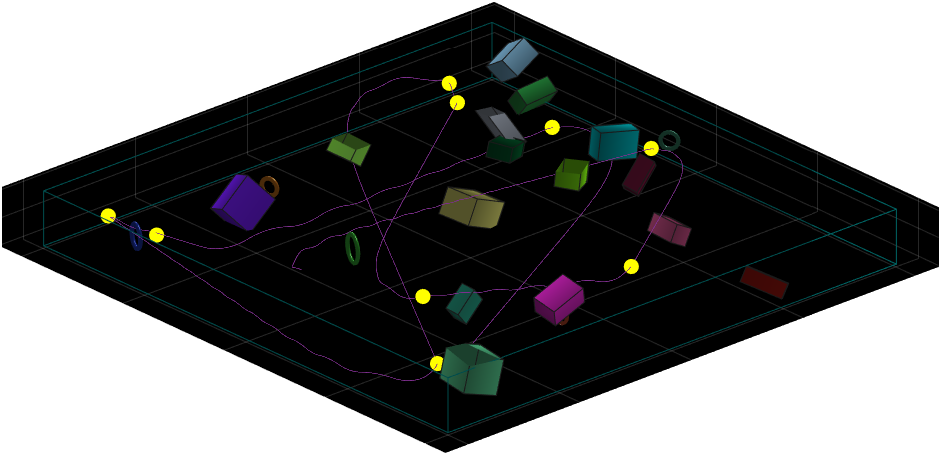
\includegraphics[scale=0.5]{Figure1}
		\caption{UAV Trajectory Through Course 1}
	\end{center}
\end{wrapfigure} 

Aside from following the project instructions, a few features were added to the simulation to make sure the UAV could get to each way point. Inside UAVControl, limits were applied to the bank angle, normalized lift and normalized thrust. Not only do those limits more accurately represent an actual flight, they made the simulation run smoother and kept the all values as real numbers. Adding additional way points made it easier for the UAV to fly to each required way point, as it wasn’t trying to turn quite so hard. In UAVRHS, limits were applied to the UAV to keep it within the boundaries of the obstacle course. 

Figure 1 shows the simulation of the UAV through Course 1 with additional way points. Running the course through the scoring function obtains an overall score of 1000 points. The UAV makes it through 2 hoops, but hits 6 cuboids. 	




\pagebreak
\subsection*{Summary of Roles}  

\begin{description}
\item[Julia Dunlop:] Wrote the UAVControl and added limits to UAVRHS to keep UAV inside course. Wrote the majority of the executive summary. 

\item[Zixin Chen:] Wrote the entire RHS function. Revised and made extra comments on the code.

\item[Peter Hartford:] Wrote the ODENumIntRK4 function, formatted the executive summary, and wrote the main report. 

\item[Trevor Burgoyne:] Meshed the functions together to get the simulation to work. Edited the parameters of the UAVControl function to get it to output reasonable values.

\end{description}

\pagebreak  
\subsection*{Report} 
The simulation was run on three different courses and scored using the ScoreUAVObstacleCourse function. 
The task of simulating the UAV simulation required a few functions to be written and modified in order for it to work properly. A brief description of each of the written functions is as follows: 
\begin{description}
	\item[PlotUAVObstacleCourse] takes in a way point list, initializes the state vector, control gains, UAV parameters, engine time response, then calls UAVFlyWaypointSequence.
	\item[UAVFlyWaypointSequence] loops through each way point to set parameters for each segment between those waypoints and calls UAVFlyToWayPoint
	\item[UAVFlyToWaypoint] sets a time interval for the segment and calls 
	UAVSim. 
	\item[UAVSim] calls UAVGuidance, which calculates the required state for the UAV to get to the next way point. 
	\item[UAVControl] takes the current state, commanded state and gain parameters and outputs the required bank angle, normalized lift, and normalized thrust.
	\item[UAVRHS] contains the dynamic model outputting the state derivatives, and is called after UAVControl inside UAVSim. The state is then updated and then the next time step is simulated. 
	\item[stopSim] breaks UAVSim when the UAV is incapable of reaching the way point due to control limits, or if the UAV passes through the way point. 
\end{description}

The control limits were edited to ensure that the UAV was ran through the course in a realistic manner. 

\end{document}